\documentclass[a4paper, 12pt]{article}				

%============== Русский язык ===============================

\usepackage[utf8]{inputenc}	
\usepackage[english,russian]{babel}	
\usepackage{multicol}
\usepackage{minted}

%============== Всякие пакеты ===============================
% нужно поставить pygments - $ sudo pip install pygments
\usepackage{listings, minted, chngcntr, float, amsmath, amssymb, cmap, graphicx, xcolor, hyperref, geometry}

 \geometry{
 	a4paper,
 	total={210mm,297mm},
 	left=10mm,
 	right=10mm,
 	top=20mm,
 	bottom=20mm,
 }
 
 \usepackage{fancyhdr}
\pagestyle{fancy}
\fancyhead{}
\fancyfoot{}
\fancyfoot[RO,LE]{
\line(1,0){570}
~~~~~~~~~~~~~ MIPT MIPT Machine Learning Practical Course
							$\bullet$ Ashuha Arseniy $\bullet$ \today}

\author{}
\date{}


%============== Цветные гиперссылки =========================
\definecolor{wine-stain}{rgb}{1,0,0}
\hypersetup{colorlinks, linkcolor=wine-stain, linktoc=all}

%============== Настройка листингов =========================
\usemintedstyle{default}
\definecolor{codebg}{rgb}{0.96,0.96,0.96}

\renewcommand\listoflistingscaption{Листинги}
\renewcommand\listingscaption{Листинг}

% === Это магия, чтоб все с рускими буквами хорошо в листиге было
% === Это макрос, чтоб не писать рараметры каждый раз

\makeatletter
\newenvironment{mycode}[3]
{\VerbatimEnvironment
	\minted@resetoptions
	\setkeys{minted@opt}{bgcolor=codebg, linenos=true, frame=lines, numbersep=5pt, tabsize=4}
	\renewcommand{\minted@proglang}[1]{#1}
	\begin{listing}[H]%% default placing
		\centering
		\caption{#2}\label{#3}
		\begin{VerbatimOut}{\jobname.pyg}}
		{\end{VerbatimOut}
		\minted@pygmentize{\minted@proglang{}}
		\DeleteFile{\jobname.pyg}
	\end{listing}}
	\makeatother
%================ Всякое разное форматирование ========================

\parindent=0cm
\title{MIPT HW 4}
%===================================================================
%===================================================================
%===================================================================
%===================================================================

\begin{document}


  \begin{center}
    \textsc{\textbf{
    	{\Large Машинное Обучение МФТИ \\
        \vspace{0.5cm}
    	Семинар: Определение Возраста}}}
  \end{center}

\begin{center}
	
\includegraphics[scale=0.9]{front_page}
\end{center}

\section*{Концепция}
	\begin{enumerate}
		\item Основная идея этой серии семинаров -- провести студентов от цели принести пользу компании (заработать денег) и наличиях каких-то данных к: постановке задаче, сбору данных, построению решения с использованием алгоритмов машинного обучения грамотному измерению качества и выкатке решен ия в продакшен. 
		
		\item Такой семинар предворяет контест, на реальных данных., где студенты смогут попробовать обсужденные на семинаре подходы к решению задачи. 
		
		\item Семинар обязательно должен проходить в формате диалога, студенты должны думать что все придумали сами. А задача семинариста их за ручку провести через это =)
		\item Семинары будет состоять из 6 основных блоков
		\begin{enumerate}
			\item Вы датасаинтесты и у вас есть данные, как заработать денег?
			\item Как свести это к задаче машинного обучения? 
			\item Откуда взять разметку?
			\item Думаем как решить задачу (в командах), обсуждаем, находим баги (самая жирная часть)
			\item Как измерить качество?
			\item Как катить в прродакшен?  (Второе дно) 
		\end{enumerate}
	\end{enumerate}

\section*{План семинара}
\begin{enumerate}
\item Вы работаете датасаинтастами в крупной интернет компании, к примеру Гугл, и у вас есть сервис аналитики. 
\item  Сервис аналитики, это такая штука которая ставит вам куку(\href{https://en.wikipedia.org/wiki/HTTP_cookie}{en.wikipedia.org/wiki/HTTP\_cookie}) в браузер, а дальше видит, на какие странички ходил человек с такой кукой.
\item  Что значит видит?  -- Есть страничка и на есть урл и заголовок(тайтл) и человек заходит на страничку в какой-то момент времени, соответственно одна транзакция, это строка \texttt{user\_id, url, title, time}

\begin{center}
	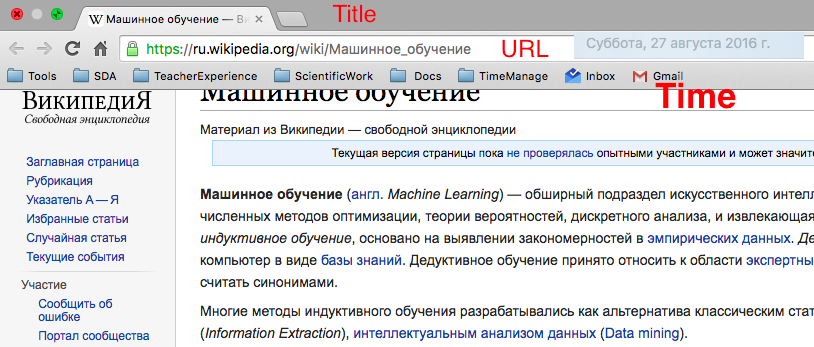
\includegraphics[scale=0.4]{br}
\end{center}

\item \textbf{Вопрос + командная работа} Как заработать денег используя эти данные?

Возможные варианта ответа:
\begin{enumerate}
	\item Показывать персоанализированную рекламу
	\item Рекомендовать хороший контент, чтобы пользователь проводил больше времени на сайте и показывать рекламу в это время
	\item ...
\end{enumerate}
\item \textbf{Убеждение} Дальше всех нужно убедить в таком сценарии, что приходят к тебе рекламу покупать, и говорят мы хотим продавать вне-дорожники от 100к\$ ценой, кто их купит -- ответ мужик старше 40 лет с большим доходом. Ну и во! Нам нужно уметь знать про людей пол возраста и доход. Давайте начнем с пола.
\item  \textbf{Вопрос + командная работа (ответ придумывают студенты)} Как решить эту задачу методами машинного обучения?
\begin{enumerate}
	\item Без учителя и набрать правил руками -- не выйдет, очень плохое решение
	\item Надо собрать обучающих данных, как???!!
	\item А у большой компании есть почта в которой все указывают пол возраст, что там еще?
\end{enumerate}
\item Супер у на есть признаки и метки, давайте к машинному обучению
\begin{enumerate}
	\item Какую задачу решать классификация регрессия, можно-ли и так и так?
	\item Какие фичи? Какие методы использовать? 
	\item Почему все что вы придумали будет работать плохо
	\begin{enumerate}
		\item Линейные модели, Голые деревья -- бесполезно, зато очень быстро учатся
		\item Скорее всего у вас мешок урлов -- это очень здоровая матрица
		\item Бустинг и Форест  на голых данных (а какой размерности у нас матрица?) будет учиться очень долго, очень много признаков -- переобучитя, низкая обобщающая способность,
		\item Сжимать признаки, хмм хороший вариант (а какой размерности у нас матрица? ) чем вы ее сожмете? -- Очень большая, ничем интеллектуальным типа svd и t-sne 
		\item На самом деле можно, но надо учиться на подбвыборках 
	\end{enumerate}
	\item попробовали Бустинг и Форест -- не работает, линейные модели плохо, сжимать svd не можем. Что делать?
	\item Давайте придумаем свои способы пожать пространство 
		\begin{enumerate}
			\item Хешинг трик
			\item Отсортировать от признаки по частоте заходов от младших к старшим и разбить на интервалы
			\item Что там еще?
			\item Какие минусы у этих подходов и как их устранить --не учитываем порядок фичей и прочее RNN, word2vec
		\end{enumerate}
	\item как адаптировать к много-классовой классификации -- возрастных груп штук 5 точно хватить
	\item сбалансирован ли датасет?
	\item Ну отлично, что-то сделали, как качество мерить, в итоге:
	\begin{enumerate}
		\item как построить процес кросс-валидации? -- использовать для теста аудитория сайта где рекламу будем показывать, разные модели на разных сайтах затащат
		\item регрессия не интерпретируема давайте на классификации мериться 
		\item Как мерить многоклассовую -- ну да есть варианты, но давайте измерим лучше качество бинарнах задач?
		\item f1 -- не объяснить боссу, точность полнота приятнее 
		\item давайте мерить полноту на заданном уровне точности
	\end{enumerate}
	\item Как катить в продакшен? Что считать в онлайне а что хранить в быстрой базе данных? Сколько у нас вообще данные? как быстро должны отвечать.
	\item Применять модель один раз за сутки, результаты в быструю базу данных, мап-редюс?
	\end{enumerate}
\end{enumerate}

	
\end{document}